\documentclass[dvipdfmx,a4paper,12pt]{article}

%% Standard
\usepackage[ngerman]{babel} 
\usepackage[utf8]{inputenc}
\usepackage[T1]{fontenc}

%% Mathe
\usepackage{amsmath}
\usepackage{amssymb}
\usepackage{amsthm}
\usepackage{latexsym}

%% Aufzaehlungen
\usepackage{enumerate}

%% Bilder
\usepackage{subfigure}
\usepackage{graphicx}

%% Absaetze usw
\usepackage{multicol}   
% zu verwenden mit 
% \begin{multicols}{$$Spaltenanzahl$$} 
%  text...
% \end{multicols}

%\setlength{\parindent}{0pt}    %Absatz-Einrueckung
%\setlength{\parskip}{3pt}      %Absatz-Abstaende


%% Fusszeilen
\usepackage{fancyhdr}
\pagestyle{fancy}
\renewcommand{\headrulewidth}{0pt}
\renewcommand{\footrulewidth}{0.4pt}
\lfoot{\NAME : \TITEL}
\cfoot{}
\rfoot{\thepage}
\lhead{}
\chead{}
\rhead{}
%\setlength{\headheight}{15pt}


%% Links
\usepackage[colorlinks=true,linkcolor=black,citecolor=black,%
bookmarksnumbered=true,breaklinks=true,pdfstartview=FitH]{hyperref}

%% Eigene Kommandos
% Differenzialrechnung
\newcommand{\diff}{\ensuremath{\mathrm d}}
\newcommand{\dx}{\ensuremath{\mathrm dx}}
\newcommand{\dvx}{\ensuremath{\mathrm d \vec x}}

% Lineares
\newcommand{\Mat}[1]{\ensuremath{\mathbf{#1}}}
\newcommand{\Ten}[1]{\ensuremath{\mathcal{#1}}}
\newcommand{\Ve}[1]{\ensuremath{\vec{#1}}}
% Vektoren sind Fette buchstaben
\renewcommand{\vec}[1]{\ensuremath{\boldsymbol{#1}}}
% Vektoren sind fett und nicht kursiv
% \renewcommand{\vec}[1]{\ensuremath{\mathbf{#1}}}
\newcommand{\skp}[2]{\ensuremath{\langle #1 \,|\, #2 \, \rangle}}


% Euler
\newcommand{\e}{\ensuremath{\operatorname{e}}}
\newcommand{\E}{\ensuremath{\operatorname{e}}}
\newcommand{\ir}{\ensuremath{\operatorname{i}}}
\newcommand{\I}{\ensuremath{\operatorname{i}}}

% allg Mathe
\newcommand{\R}{\ensuremath{\mathbb{R}}}
\newcommand{\folgt}{\ensuremath{\Rightarrow}}
\newcommand{\gdw}{\ensuremath{\Leftrightarrow}}


% Formatierung
\newcommand{\abs}[0]{\bigskip\noindent}
\newcommand{\const}{\ensuremath{\text{\emph{const}}}}


% Umgebungen
\newtheorem{satz}{Satz}[section]
\newtheorem{defi}{Definition}[section]
\newtheorem{lemma}{Lemma}[section]






\begin{document}



\newcommand{\NAME}{Michael Kopp}
\newcommand{\FACH}{Weiche Materie}
\newcommand{\TITEL}{Blatt 06, Aufgabe 2:\emph{TIRM}}
\newcommand{\DATUM}{\today}


\pagestyle{plain} 
	% auskommentieren fuer fusszeile



%%%% Eigener Kopf

\sloppy

\begin{center}
\FACH
\hfill
\DATUM
\end{center}

\vspace{-5mm} % weniger abstand

\begin{center}
  \begin{Large}
 \textbf{\TITEL}
  \end{Large}
\end{center}

\vspace{-3mm}

\begin{center}
\hrulefill
%\quad
 %\raisebox{-1.5mm}{\NAME}
% \,
\quad 
\textit{\NAME}
\,
\hrulefill
\end{center}
 
 
%%%%%%%%%%%%%%%%%%%%%%%%%%%%%
%%%%%%%%%%%%%%%%%%%%%%%%%%%%%%
%%%%%%%%%%%%%%%%%%%%%%%%%%%%%%%%

 
\noindent
Gegeben ist ein Datensatz $I(t)$ und der Zusammenhang
\begin{equation}
  I(z) = I_0 \exp( - \beta z) \gdw
  z(I) - z_0 = - \frac{1}{\beta} \ln I
  \label{eq:Iz}
\end{equation}
mit $z_0 = \ln{ I_0 }/\beta$, sodass man aus dem Datensatz $z(t)=z(I(t))$ gewinnen kann.

Um daraus eine Verteilungswahrscheinlichkeit $P(z-z_0)$ zu generieren, bildet man ein Histogramm mit allen so erhaltenen $z$-Werten. Dies ist in Abb. \ref{fig:histo} dargestellt.


Um daraus das Potential $\phi = \phi(z)$ zu bestimmen, verwendet man
\begin{equation}
  P(z-z_0) = P_0 \exp\left( - \frac{\phi(z-z_0)}{kT} \right) \gdw
  \frac{\phi(z-z_0) - \varphi_0}{k T}= - \ln {P(z-z_0)}
  \label{eq:phi}
\end{equation}
mit $\varphi_0 = k T \ln P_0$, was in Abb.  \ref{fig:pot} dargestellt ist.

Offenbar stimmt dieses Potential\footnote{besonders, wenn man nur Werte $z-z_0 < 0.3$ beachtet} hervorranged mit dem von Doppellagenkr"aften ($\phi_1 \propto \exp(-z)$), "uberlagert durch die Schwerkraft ($\phi_2 \propto z$) "uberein -- siehe die Fits in \ref{fig:pot}.

 
\begin{figure}[h]
  \begin{center}
    \subfigure[Histogramm f"ur $z-z_0$; 100 Bins.]{\label{fig:histo}\includegraphics[width=0.45\textwidth]{./histo}}
    \subfigure[Potential $\phi$ aus Histogramm.]{\label{fig:pot}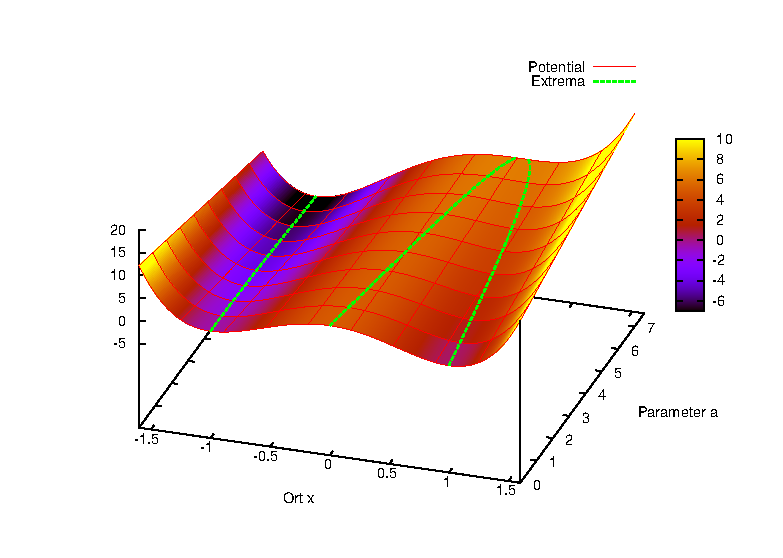
\includegraphics[width=0.45\textwidth]{./pot}}
  \end{center}
  \caption{Auswertung der gegebenben Daten $I(t)$.}
\end{figure}
 
 
 
 
 
 
 



\end{document}

